\chapter{Evaluating the influence of local sequence context on rates of mutation}
\label{chpt:lsci}

Germline mutation, the primary source of heritable genetic 
variation, is an inherently stochastic process which introduces 
approximately $1-1.5 \times 10^{-8}$ 
mutations per base pair per generation in humans \citep{rahbari2015}. 
The rate at which these mutations occur across the genome is not uniform, and this variation has been previously shown to be associated with genomic features such as  local sequence context \citep{Aggarwala2016, Zhu2017, Carlson2018, Seplyarskiy2023}, replication timing \citep{Francioli2015}, recombination rate \citep{Lercher2002}, GC content \citep{Fryxell2004}, and epigenomic markers such as H3K9me3 peaks \citep{Schuster2012, Supek2015}. 
Mutation rate estimates play a key role in applications such as demographic history inference \citep{Li2011} and the identification of likely pathogenic mutations among candidates identified in a GWAS \citep{MacArthur2014}, but often the mutation rate is parameterized as a single value representing an average rate across the genome. 
Previous efforts to estimate a per-base mutation rate along the genome have utilized various measures of genomic and epigenomic features in their models, but for many features it is yet unclear how to best incorporate them into models of germline mutation rate variation.

A challenge in understanding the influence of local sequence context on mutation rates is in disentangling the effect of neighboring nucleotides on rates of mutation from that of other genomic features. In their evaluation of nucleotide motifs and germline mutation, \citep{Zhu2017} proposed a matched-control approach in which each variant is matched to a nearby non-variant site whose nucleotide in the reference genome matched the reference allele of the variant. In doing so, by controlling for genomic location one would also control for genomic features also associated with genomic location, yielding a set of control non variant sites affected by the same genomic features as their matched singletons. Comparisons of the distributions of nucleotides flanking genomic variants could be compared to that of their matched controls in order to identify motifs associated with mutation. The results in \citep{Zhu2017} are limited in several respects; by evaluating the distribution of nucleotides flanking common variants, their results could also reflect non-mutation processes such as natural selection and biased gc-conversion \citep{Carlson2018}. In addition, \citep{Zhu2017} were also unable to compare results across populations. Recent studies have indicated potential differences in mutation processes among different ancestry groups \citep{Harris2017, Mathieson2017}. While these studies suggest that population-level differences in mutation processes may have differed in the past, the question of whether there exist differences in these processes in modern human populations is under-explored.

Here we explore the marginal influence of local sequence context on germline mutation rates by assessing the distributions of nucleotides flanking singleton variants from the 1000 Genomes Project (1kGP) 30x deep-sequencing release. To control for the influence of other genomic and epigenomic features, we follow \citep{Zhu2017} and compare the distributions of nucleotides at positions flanking singletons to nucleotides at corresponding flanking positions of non-variant control sites matched based on proximity to the singleton variants. We evaluate the influence of nucleotides at independent positions in a +/- 1000 base pair window on rates of mutations, and the influence of pairs of nucleotides at each combination of flanking positions within 10 bases of the focal position. In addition, we assess third-order interactions within this 20-mer window as well. We assess the influence of neighboring positions in this manner for each individual 1kGP super-population along with the analysis utilizing all singletons from the 1kGP data, allowing for cross-population comparisons of the results.

With each category of singleton (defined by the reference and alternative alleles) matched to a sample of non-variant sites, we employ a log-linear model framework to compare distributions of nucleotides at flanking positions between the singletons and their matched controls, with deviances between these distributions implying the influence of nucleotides at these flanking positions on mutation rates for that subtype. For example, when we consider the distribution of nucleotides at a single flanking position, we fit the following log-linear regression model:

\begin{equation}
    \log(n_{is}) = \lambda_0 + \lambda_{i}^{\textrm{base}} + \lambda_{s}^{\textrm{status}} 
\end{equation}

What we have with this model is a total number of observations that we categorize based on: whether the observation is a singleton or a matched control ($s$), which we further stratify based on which nucleotide is observed at a given flanking position ($i$). This model is fit for all mutation subtypes at all flanking positions within 1000 positions up or downstream of the focal position.
To evaluate the influence of nucleotides at each flanking position, we compute the deviance statistic for each of these models. The deviance statistic is a measure of goodness of fit which compares the above model to a fully saturated model:

\begin{equation}
    \log(n_{is}) = \lambda_0 + \lambda_{i}^{\textrm{base}} + \lambda_{s}^{\textrm{status}} + \lambda_{i:s}^{\textrm{base:status}}
\end{equation}

The null hypothesis for this test is that $\lambda^{\textrm{base:status}}=0$ for all $i,s$, and the deviance statistic for the single position model follows a $\chi^2$ distribution with 3 degrees of freedom. To allow for comparisons among subtypes and populations, where the number of observations differ, we compute the relative entropy statistic by dividing the deviance statistic by twice the number of singletons and matched controls. 

\begin{figure}
    \centering
    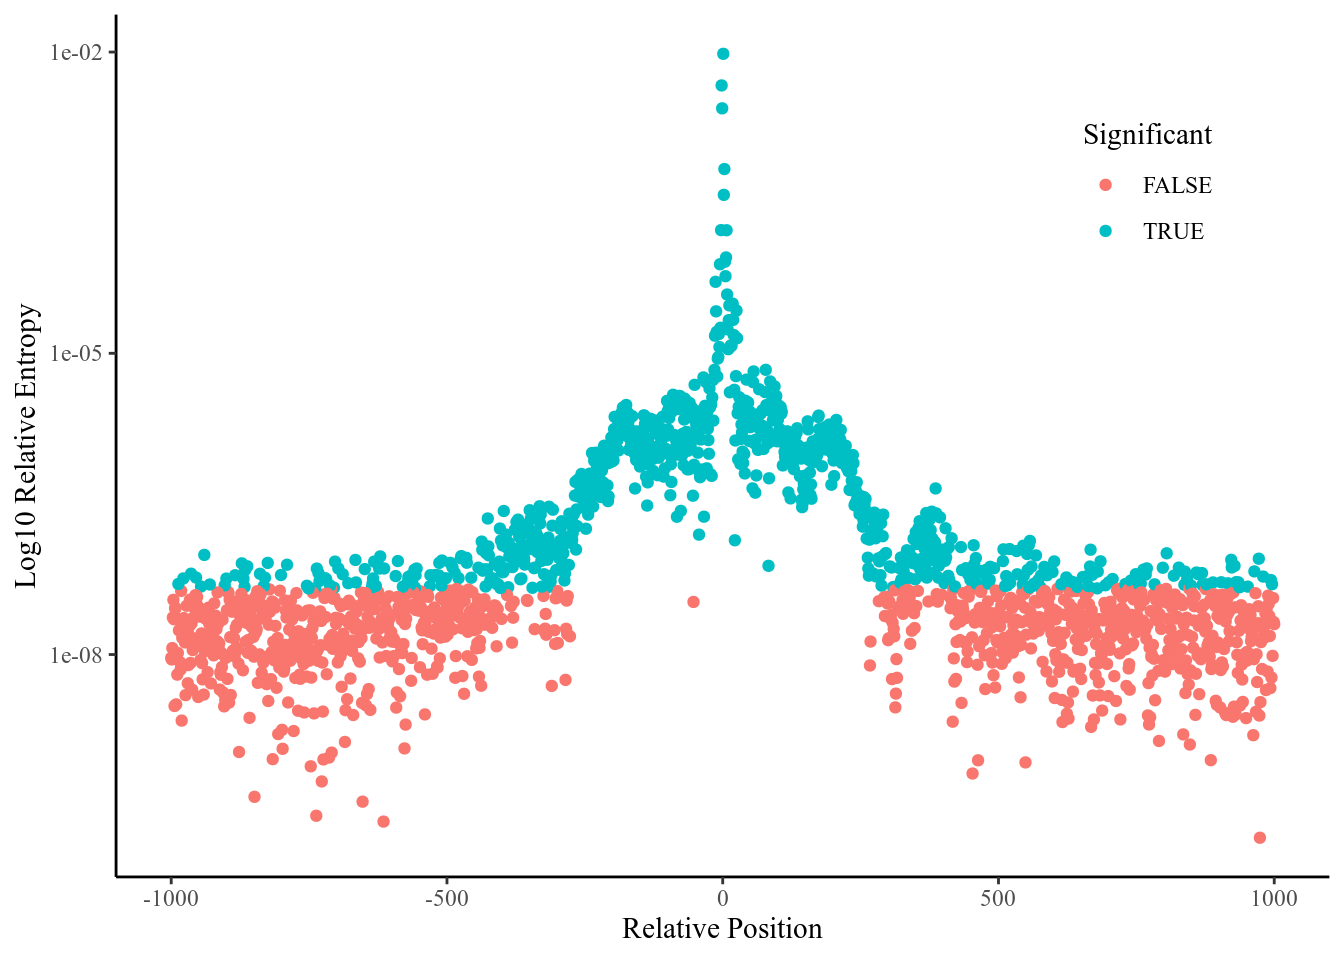
\includegraphics[scale=0.75]{chapters/figures/A_G_sp.png}
    \caption{Relative entropy statistics at individual positions flanking A $\rightarrow$ G mutations. We observe the strongest effects at positions closer to the focal position, but we find that position-level effects remain significant in a $\pm 250$ base-pair window centered at the focal position (null-distribution: $\chi^2$, df = 3).}
    \label{fig:single_pos}
\end{figure}

To assess the extent to which interactions among flanking positions influence rates of mutation for each subtype, we fit additional models which stratify counts of observations based on the nucleotides at multiple flanking positions. This is achieved by adding additional parameters to our log-linear models. As an example, to assess the influence of interactions among two given flanking positions, we fit the following log-linear regression model:

\begin{equation}
    \log(n_{i,j,s}) = \lambda_0 + \lambda_i^{\textrm{base}_1} + \lambda_j^{\textrm{base}_2}  + \lambda_s^{\textrm{status}} + \lambda_{is}^{\textrm{base}_1:\textrm{status}} + \lambda_{js}^{\textrm{base}_2:\textrm{status}} + \lambda_{ij}^{\textrm{base}_1:\textrm{base}_2}
\end{equation}

Here we account for the non-uniform distribution of dinucleotides genome-wide by including an interaction term between the bases at the two flanking positions. We also control for the effects that individual positions may have on the rate of substitution by including the interaction term between the base at each position and the singleton/control status indicator. The deviance statistic for this model compares the fit to that of a fully saturated model; the difference between the two models is the absense of a three-way interaction between the nucleotides at the two flanking positions and the singleton/control status. A significant statistic here shows that the two-way interaction between the nucleotides at the two flanking positions is different between the singletons and their matched controls, implying that the nucleotides at the two flanking positions influence each other in determining their influence on rates of mutation at the focal position.

\begin{figure}
    \centering
    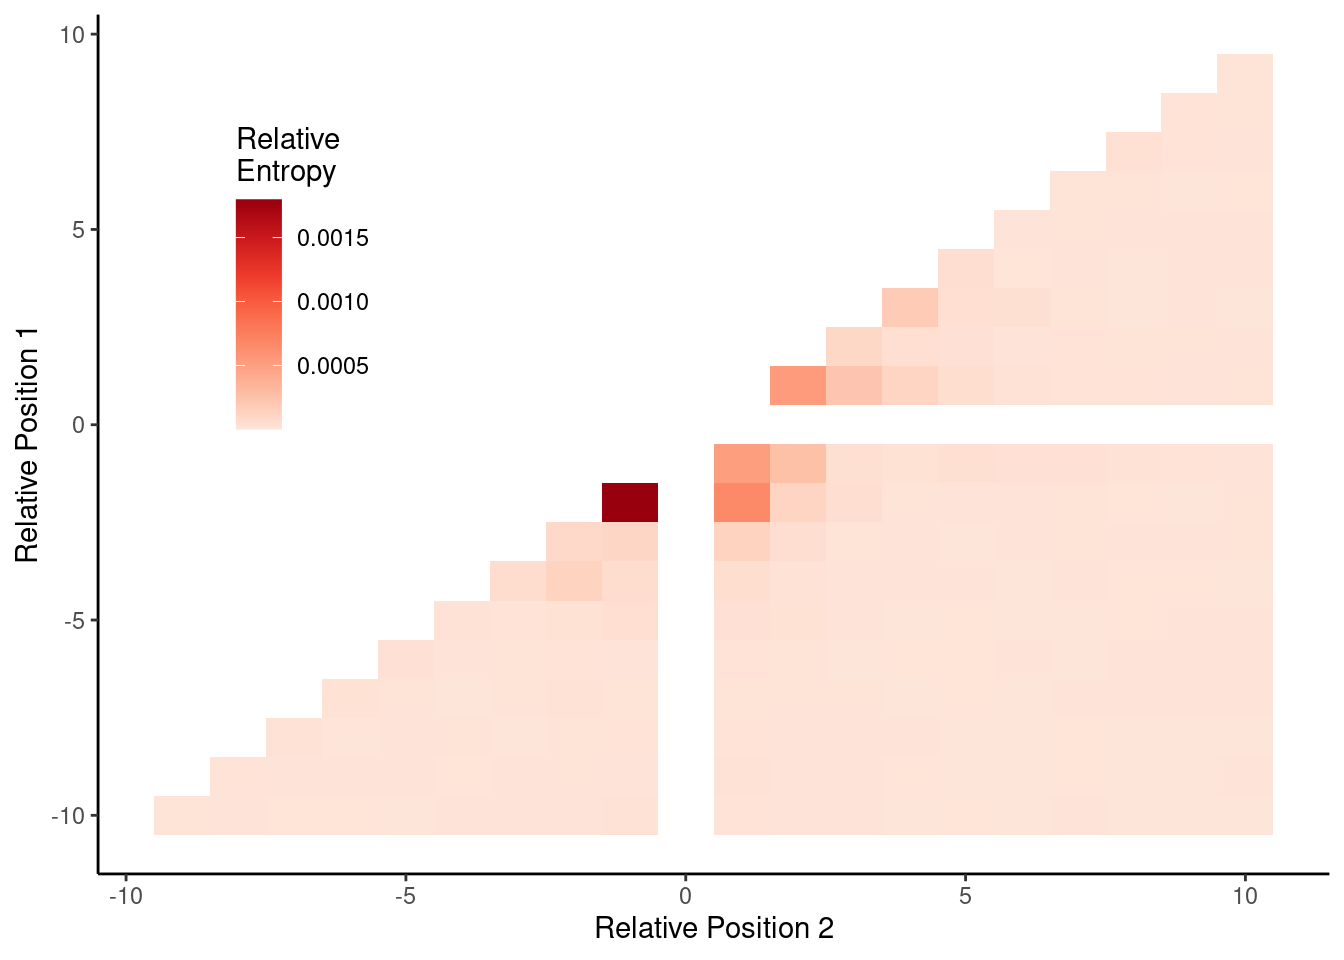
\includegraphics[scale=0.75]{chapters/figures/A_G_tp.png}
    \caption{Relative entropy statistics for two position interactions among positions flanking A $\rightarrow$ G mutations. While all interactions among pairs of flanking positions are statistically significant ($\chi^2$, df = 9), we observe the strongest interactions at pairs closer to the focal position.}
    \label{fig:two_pos}
\end{figure}

In addition to the above models for the influence of flanking nucleotides, we also assess for cross-population differences by the addition of a population term in our model. For example, the model 

$$
\log(n_{isp}) = \lambda_0 + \lambda_{i}^{\textrm{base}} + \lambda_{s}^{\textrm{status}} + \lambda_p^{\textrm{population}} + \lambda_{i:s}^{\textrm{base:status}}
$$

allows for us to assess whether single position effects for a subtype are shared between populations. The null hypothesis for this model is that there is no population-specific base-by-status interaction, and a high deviance would suggest that there are population-level differences in the nucleotide-level contributions to the overall signal at the flanking position.

